\section{Processi organizzativi}
Questa sezione mira a gestire i processi e il loro miglioramento, l'organizzazione degli strumenti
di supporto e la gestione del personale.

    \subsection{Pianificazione}
        \subsubsection{Metodo di Lavoro}
        Il team ha adottato il metodo di lavoro Scrum, una delle metodologie Agile più diffuse.
        Di conseguenza seguendo questo modello, i compiti derivanti dai processi di sviluppo vengono suddivisi in sprint che il team ha deciso
        durare due settimane.\\
        Questo rende l'avanzamento del prodotto più gestibile e più rapido, avendo però un tempo abbastanza longevo per implementare diverse
        feature e redigere i documenti necessari.
            \paragraph*{Sprint}\label{inf:sprint} ~\\\\
            Per ogni sprint, il responsabile assegna i ruoli a ciascun membro, creando un diagramma delle attività per stimare le ore
            necessarie e tenendo traccia dei giorni in cui ogni membro può contribuire alla realizzazione del progetto.
            Successivamente l'amministratore si occuperà di creare le issue associate allo sprint in modo da rendere il lavoro degli altri membri più semplice e veloce.
            Inoltre assicura che sia avvenuta la verifica, in caso di modifica, del \textit{Piano
            di Progetto} e delle \textit{Norme di Progetto} prima dell'inizio dello sprint successivo, in modo da avere sempre la
            documentazione adatta e aggiornata sotto mano.\\\\
            Le attività dello sprint sono le seguenti:
            \begin{itemize}
                \item \textbf{Sprint planning}: 
                \begin{itemize}
                    \item Il team definisce collettivamente le attività da svolgere durante lo sprint;
                    \item Ogni componente del gruppo, durante la riunione, segnala le ore che può mettere a disposizione;
                    \item Il responsabile assegna i ruoli e definisce gli obiettivi dello sprint nel documento \textit{Piano di progetto}.
                \end{itemize}
                \item \textbf{Daily Scrum}: ogni giorno, i membri del team sono tenuti a condividere, attraverso il gruppo \textit{Telegram} dedicato,
                un report dettagliato delle attività svolte il giorno precedente,
                quelle pianificate per la giornata in corso e segnalando eventuali ostacoli che potrebbero compromettere il lavoro.
                Il responsabile controlla l'andamento dello sprint contattando i componenti del gruppo.
                \item \textbf{Sprint review}:
                \begin{itemize}
                    \item Ogni membro, durante la riunione, riferisce quello che ha svolto nel periodo precedente e gli eventuali dubbi che ha riscontrato;
                    \item Viene fatta una lista degli obiettivi raggiunti e quelli non raggiunti.
                \end{itemize}
                \item \textbf{Sprint retrospective}: si fa una valutazione di quello che è andato bene durante lo sprint e di
                quello che è da migliorare, per capire come comportarsi per lo sprint successivo.
            \end{itemize}

        \subsubsection{Ruoli e responsabilità}
            I membri team \textit{Six Bit Busters} ricopriranno i ruoli principali 
            di un ciclo di vita del prodotto software, ovvero analista, 
            progettista, programmatore, verificatore, amministratore di sistema e responsabile. \\
            Al fine di garantire una comprensione completa delle diverse fasi 
            e competenze richieste nello sviluppo di un progetto, i membri del team 
            ruoteranno periodicamente tra i ruoli ogni due settimane. Questa rotazione 
            periodica è finalizzata a scopi didattici, permettendo a ciascun membro di 
            acquisire una visione globale del ciclo di vita del prodotto e di sviluppare 
            abilità pratiche in ogni area.
            \begin{itemize}
                \item \textbf{Responsabile}\\
                Colui che possiede la visione d'insieme del progetto, coordina i membri fra i vari sprint e condensa tutte le voci del team
                dialogando con il proponente per rappresentare il progetto.
                Le sue competenze sono:
                \begin{itemize}
                    \item Ad ogni sprint si ha solo un Responsabile;
                    \item Presenta il Diario di Bordo in aula;
                    \item Suddivide le attività del gruppo;
                    \item Approva i documenti prima di eseguire il merge nel branch "main", aggiornando la versione del documento e quindi andando ad incrementare il numero più a sinistra;
                    \item Redige i verbali.
                \end{itemize}
                \item \textbf{Amministratore di sistema}\\
                Colui che si occupa del funzionamento, mantenimento e sviluppo degli strumenti e ambienti tecnologici
                usati dal gruppo.
                Le sue competenze sono:
                \begin{itemize}
                    \item Ad ogni sprint si hanno al massimo due Amministratori;
                    \item Gestisce le segnalazioni e problemi dei membri del gruppo relativi a malfunzionamenti e difficoltà con gli strumenti tecnologici;
                    \item Valuta l'utilizzo di nuove tecnologie e ne fa uno studio preliminare per poter presentare al
                        gruppo i pro e i contro del suo utilizzo;
                    \item Controlla giornalmente la board e issue per garantire una buona organizzazione;
                    \item Controlla se la documentazione è aggiornata;
                    \item Redige i verbali nel caso in cui il responsabile sia impossibilitato.
                    \end{itemize}
                    \item \textbf{Analista}\\
                    Colui che si occupa di analizzare a fondo il capitolato e le richieste del proponente per estrarne i requisiti.
                    Le sue competenze sono:
                    \begin{itemize}
                        \item Ad ogni sprint si hanno almeno 2 Analisti;
                        \item Studia le risposte e richieste del proponente per identificare i requisiti e redigere l' Analisi dei Requisiti.
                    \end{itemize}
                    \item \textbf{Progettista}\\
                    Colui che trasforma i requisiti, ricavati degli analisti, in una soluzione che abbia bassa complessità individuale.
                    Le sue competenze sono:
                    \begin{itemize}
                        \item Sceglie eventuali pattern architetturali da implementare;
                        \item Sviluppa lo schema UML delle classi.
                    \end{itemize}
                    \item \textbf{Programmatore}\\
                    Colui che si occupa di realizzare tramite codice il design presentato dal progettista.
                    Le sue competenze sono:
                    \begin{itemize}
                        \item Scrive il codice atto a implementare lo schema delle classi;
                        \item Scrive eventuali test per il codice;
                        \item Scrive la documentazione per la comprensione del codice che scrive.
                    \end{itemize}
                    \item \textbf{Verificatore}\\
                    Colui che si occupa a verificare/controllare che ogni file rispetti le \textit{Norme di Progetto} prima che sia caricato in un branch protetto.
                    Le sue competenze sono:
                    \begin{itemize}
                        \item Controlla che la documentazione e il codice scritto siano conformi alle \textit{Norme di progetto};
                        \item Propone possibili migliorie da apportare a documenti e/o codice tramite dei commenti, non li può modificare direttamente.
                    \end{itemize}
            \end{itemize}

            Per l'analisi dei ruoli e la rendicontazione delle ore preventivate si faccia riferimento al documento \textit{Dichiarazione degli impegni}.

    \subsection{Modalità di comunicazione}
        \subsubsection{Interne}
        Si svolgono tra i componenti del gruppo tramite diversi canali di comunicazione.\\
        Si è deciso di utilizzare:
        \begin{itemize}
            \item \textbf{Telegram}: canale di comunicazione asincrono per comunicazioni brevi e poco importanti;
            \item \textbf{Discord}: canale di comunicazione sincrono per le riunioni con i soli membri del team.\\ 
        \end{itemize}
        \subsubsection{Esterne}
        Si svolgono tra il gruppo e una persona esterna, generalmente il proponente.
        Si è deciso di utilizzare:
        \begin{itemize}
            \item \textbf{Google Chat}: per messaggi brevi e per organizzare delle riunioni, scritti dal responsabile;
            \item \textbf{Google Meet}: per riunioni in videochiamata. Queste riunioni dovranno essere richieste
            dal gruppo e al termine verrà redatto un Verbale.
        \end{itemize}


    \subsection{Modalità di riunione}
        \subsubsection{Interne}
        Le riunioni interne si svolgono esclusivamente tra i membri del gruppo utilizzando il canale apposito
        del server \textit{Discord}.\\
        Per ogni riunione il responsabile sarà incaricato di:
        \begin{itemize}
            \item Preparare una scaletta degli argomenti da trattare, che potranno essere poi integrati da eventuali
            punti di discussione portati dagli altri membri del gruppo;
            \item Scrivere il verbale interno a fine riunione.
        \end{itemize}

        Le riunioni si svolgeranno a cadenza settimanale, cercando di trovare giorni e orari agevoli a tutti i
        membri del gruppo.

        \subsubsection{Esterne}
        Le riunioni esterne si svolgono tra i membri del gruppo e il proponente a cadenza bisettimanale,
        dove al termine della riunione verrà redatto un verbale esterno.

    \subsection{Gestione di Infrastrutture}
        \subsubsection{Descrizione}
        In questa sezione sono riportate le norme relative alla gestione delle infrastrutture, vengono stabiliti gli
        strumenti di cui il gruppo farà uso e le relative regole di utilizzo.

        \subsubsection{GitHub}
        Come servizio di hosting per il progetto il team ha optato per GitHub. 
        Oltre alla copia in remoto del repository di progetto ogni componente del gruppo ha una propria
        copia in locale nella quale può testare e fare prove senza compromettere la struttura del progetto.
        Per prove più complesse è consigliabile eseguire un fork della repository, in modo tale da avere una copia uno ad uno anche in 
        remoto sul proprio account personale.\\
        Per ottenere una copia del repository ogni componente deve scaricarla utilizzando Git ed eseguendo uno dei due comandi 
        su git bash o terminale windows:
        \begin{verbatim}
            git clone <git@github.com:6BitBusters/6BitBusters.github.io.git>
            git clone <https://github.com/6BitBusters/6BitBusters.github.io.git>
        \end{verbatim}
        Il primo se si usano le ssh key per l'autenticazione, il secondo se si usano i personal token.\\
        Una volta completato il download verrà creata una cartella collegata alla repository del progetto in remoto.\\
        I componenti del gruppo abituati ad interagire con GitHub da interfaccia grafica possono continuare a
        farne uso.
        
        \subsubsection{Overleaf}
        Inizialmente il team aveva deciso ad utilizzare \textit{Overleaf} come text editor principale per la scrittura di documenti online utilizzando \textit{LaTeX}, successivamente ci siamo accorti
        che non era un modo ottimale per creare documenti avendo anche implementato un'automazione di build direttamente su GitHub.
        In questo momento \textit{Overleaf} è utilizzato solamente come text editor di appoggio, per chi non vuole installare \textit{LiveTex} in locale.
        
        
        \subsubsection{Repository}
        Il repository si può trovare all'indirizzo \textbf{\url{https://githubg.com/6bitbusters/6bitbusters.github.io}} ed è pubblico.
        I collaboratori sono i componenti del gruppo \textit{6BitBusters} che utilizzano il proprio account GitHub
        personale per collaborare al progetto.
        La struttura del repository è formata in questo modo:
            \begin{itemize}
                \item \textbf{ .github}: cartella che contiene i file sorgenti delle GitHub Action e template per le issue;
                \item \textbf{3Dataviz}: cartella che contiene i file sorgente del prodotto;
                \item \textbf{Docs}: cartella che contiene la documentazione, si divide ulteriormente in:
                    \begin{itemize}
                        \item \textbf{Candidatura}: cartella che contiene i documenti da presentare per la candidatura;
                        \item \textbf{Generali}: cartella che contiene tutta la documentazione esterna e interna tranne i verbali;
                        \item \textbf{Verbali esterni}: cartella contenente i verbali esterni, che riportano gli incontri con i proponenti;
                        \item \textbf{Verbali interni}: cartella contenente i verbali interni, relativi agli incontri tra membri del gruppo.
                    \end{itemize}
                \item \textbf{website}: cartella che contiene i file sorgente del sito web che successivamente verrà pubblicato utilizzando GitHub Pages.
            \end{itemize}
        Infine il repository è dotato di sistema di auto-build per la documentazione grazie alle GitHub Actions. Nello specifico sono stati scritti 2 tipi di Action
        \begin{itemize}
            \item Per il push sul branch "main" che ha il compito di compilare tutta la documentazione creata fino a quel momento e di \textbf{creare la page};
            \item Per un test di compilazione solamente della parte aggiunta nel branch derivato, questo test deve essere \textbf{passato con successo} in modo da sbloccare l'azione di merge.
        \end{itemize}
        Per maggiori informazioni riguardanti i branch seguire le regole descritte nella sezione \nameref{inf:branch}

        \subsubsection{Branching}\label{inf:branch}
        I branch si dividono in:
        \begin{itemize}
            \item \textbf{Branches protetti}: 
            \begin{itemize}
                \item \textbf{main}: branch principale che contiene la documentazione e codice approvato del responsabile, non che la parte che viene mostrata sulla page;
                \item \textbf{docs/NOME-DOCUMENTO}: sono più branch che contengono solamente le versioni di documenti verificate;\\
                Il nome di questi branch deve essere:
                \begin{center}
                    \textbf{\textit{docs/[NOME-DOCUMENTO]}}
                \end{center}
                dove:
                \begin{itemize}
                    \item \textbf{NOME-DOCUMENTO}: indica il nome del documento in questione.
                \end{itemize}
            \end{itemize}
            \item \textbf{Branches derivati}: sono branch utilizzati per aggiungere modifiche e aggiornare un documento o una parte di codice che poi dovrà essere verificata
            attraverso una Pull Request verso il branch da cui esso è stato derivato;\\
            I nomi di questi branch, per quanto riguarda la documentazione, si suddividono in 2 casi:
            \begin{itemize}
                \item \textbf{Per Verbali e Glossario}:
                \begin{center}
                    \textbf{\textit{docs/[NOME-DOCUMENTO]-[COGNOME-ASSEGNATARIO]}}
                \end{center}
                \item \textbf{Per tutto il resto della documentazione}:
                \begin{center}
                    \textbf{\textit{docs/[NOME-DOCUMENTO]-[ID-ISSUE]}}
                \end{center}
            \end{itemize}
            dove:
    
            \begin{itemize}
                \item \textbf{NOME-DOCUMENTO}: indica il nome del documento sul quale si sta lavorando;
                \item \textbf{ID-ISSUE}: indica il numero identificativo associato alla issue relativa alla modifica del documento;
                \item \textbf{COGNOME-ASSEGNATARIO}: indica il cognome del membro che ha redatto il documento.
            \end{itemize}
            Nel caso un componente volesse richiedere una Pull Request ma il branch di destinazione fosse più aggiornato di quello di partenza o derivato, il branch protection
            impone che avvenga un merge dal branch di destinazione a quello di partenza in modo tale da applicare le modifiche delle versioni già approvate, al documento, che ne contiene
            altre e che di conseguenza deve passare ad una versione successiva.
            \item \textbf{Branch di hotfix}: sono branch dedicati all'hotfix e quindi a correzioni minime, sia per la documentazione che per il codice. Valgono le stesse regole dei
            branch protetti, quindi le modifiche devono essere sempre verificate e in caso approvate.
            Il nome per questi branch deve essere:
            \begin{center}
                \textbf{\textit{hotfix/[NOME-DOCUMENTO]}}
            \end{center}
            dove:

            \begin{itemize}
                \item \textbf{NOME-DOCUMENTO}: indica il nome del documento che viene modificato.
            \end{itemize}
        \end{itemize}

        In ogni branch secondario il lavoro può essere svolto da un solo componente del gruppo, specificatamente colui che ha preso in carico l'issue alla cui risoluzione quel branch è dedicato.
        È tuttavia possibile assegnare una issue a più persone; in tal caso, a ciascun assegnatario verrà dedicato un branch su cui lavorare. Al termine delle modifiche, prima di aprire la Pull Request 
        per la verifica del lavoro svolto, sarà necessario eseguire il merge dei vari branch secondari tramite una Pull Request specifica. Quest'ultima non richiederà ulteriori verifiche, poiché tali attività
        saranno eseguite nell'apposita Pull Request destinata a questo scopo.
    
         
        Una volta che la issue viene risolta il componente deve richiedere una Pull Request
        verso il branch da cui esso è stato derivato.
        Notare che se il branch di destinazione è:
        \begin{itemize}
            \item \textbf{main} $\rightarrow$ il documento deve essere approvato;
            \item \textbf{docs/NOME-DOCUMENTO} $\rightarrow$ il documento deve essere verificato e successivamente viene eliminato il branch derivato.
        \end{itemize}

        Di seguito si riporta un semplice ma esaustivo workflow tramite immagine:
        \begin{center}
            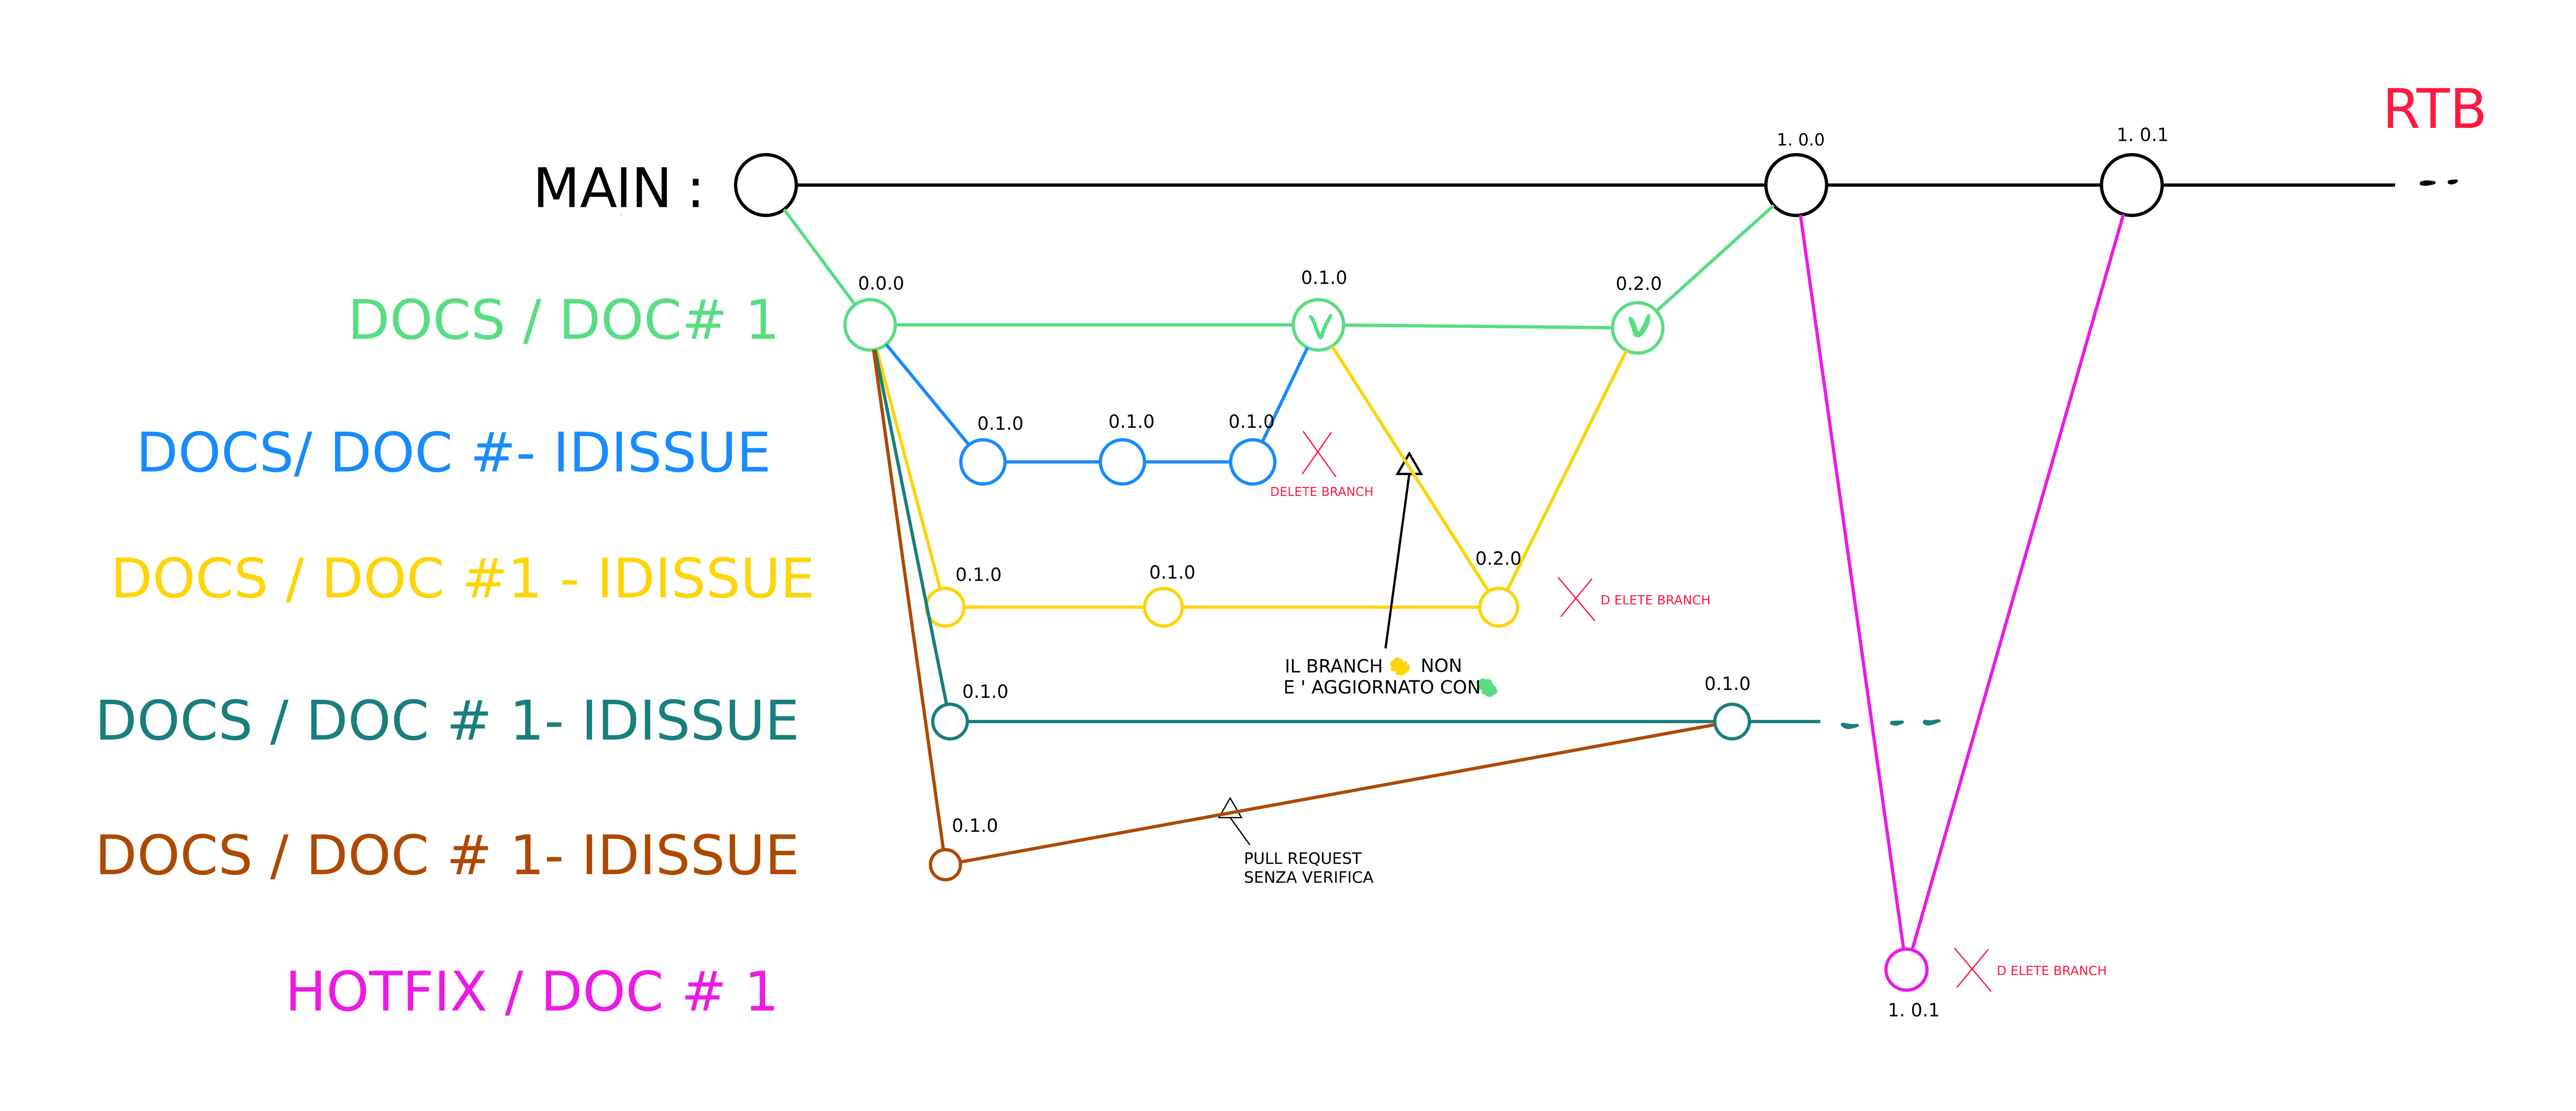
\includegraphics[scale = 0.07]{template/images/workflow.jpg}
        \end{center}

        \subsubsection{Commits}\label{inf:comm}
        E'preferibile che ogni commit abbia una singola responsabilità per cambiamento.
        I commits non possono essere effettuati direttamente sui branch protetti ma per contribuire con delle aggiunte o
        modifiche sarà necessario aprire una Pull Request, motivo per il quale abbiamo introdotto dei branch derivati.
        I messaggi di commit dovranno seguire la seguenti strutture sintattiche:
        \begin{center}
            \textbf{add: [NOME-DOCUMENTO]-[ID-ISSUE]\\
            change: [COSA]\\
            restructure: [COSA]}
        \end{center}
        dove: 
        \begin{itemize}
            \item \textbf{add}: viene utilizzato per il primo un primo commit;
            \item \textbf{change}: per i successivi commit, nei quali si va a modificare il documento già esistente;
            \item \textbf{restructure}: indica una ristrutturazione del branch main per quanto riguarda l'organizzazione delle cartelle e/o la modifica di action o template di issue;
            \item \textbf{NOME-DOCUMENTO}: indica il nome del documento creato;
            \item \textbf{NOME-SEZIONE}: indica la sezione relativa al documento creato;
            \item \textbf{COSA}: breve descrizione di cosa di è aggiunto e/o fatto.
        \end{itemize}

        Notare però che dopo l'approvazione di una Pull Request tutti i commit
        relativi verranno raggruppati in un unico commit, il quale titolo deve rispettare la struttura sintattica descritta in
        seguito.
        \begin{center}
            \textbf{Update: [NOME-DOCUMENTO] to [VERSONE]}
        \end{center}
        dove:

        \begin{itemize}
            \item \textbf{NOME-DOCUMENTO}: indica il nome del documento nel quale sono state verificate le modifiche;
            \item \textbf{VERSIONE}: indica il numero di versione aggiornata.
        \end{itemize}
        Per quanto riguarda il commento facoltativo, si lascia quello di default proposto da GitHub, ovvero un elenco puntato di tutti i commit che verranno raggruppate.\\
        

        Per aggiornare direttamente il main si è deciso di disabilitare temporaneamente
        il protection, eseguire un commit con delle modifiche, con la struttura sintattica elencata sopra, e in fine attivare nuovamente il protection.
        Questa soluzione è stata adottata perché il team ritiene sia più veloce e semplice apportare modifiche a template e action in questo modo
        rispetto che alla creazione di un branch e ad un successivo Pull Request, inoltre il branch main una volta ultimate le automazioni non verrà più modificato se non dai merge
        scatenati delle Pull Request.

        \subsubsection{Pull requests}\label{inf:pr}
        Per effettuare un merge su un branch protetto si deve aprire, da GitHub, una Pull Request. Questa
        permette di verificare il lavoro svolto prima di integrarlo con un branch protetto ed eseguire un veloce test di compilazione della sezione aggiunta.
        Alla creazione di una Pull Request bisogna associare:
        \begin{itemize}
            \item \textbf{Title}: [NOME-DOCUMENTO]-[NOME-SEZIONE];
            \item \textbf{Verificatori in carica}: hanno il compito di trovare eventuali errori o mancanze e fornire un feedback
            riguardante il contenuto direttamente su GitHub attraverso un commento, sulla stessa Pull Request.
            Non sarà possibile effettuare il merge finché tutti i commenti di revisione non saranno stati risolti
            con, al termine, l'approvazione di almeno uno dei verificatori e il test di build non dia esito positivo;
            \item \textbf{Descrizione}: contiene una lista riassuntiva di cio' che è stato fatto includendo le issue completate, e quindi da chiudere,
            con la sintassi
            \begin{center}
                \textbf{\textit{close ID-ISSUE}}
            \end{center}
            in modo tale che vengano tutte chiuse in automatico quando la Pull request verrà accettata;
            \item \textbf{Gli assegnatari}: coloro che hanno anche il compito di apportare le modifiche necessarie al documento;
            \item \textbf{Labels}: che riassumono di che natura è la Pull Request.
        \end{itemize}
        dove:

        \begin{itemize}
            \item \textbf{NOME-DOCUMENTO}: indica il nome del documento sul quale si sta lavorando e richiedendo l'approvazione;
            \item \textbf{NOME-SEZIONE}: indica la sezione relativa al documento creato;
            \item \textbf{ID-ISSUE}: indica il numero identificativo associato alla issue relativa alla modifica del documento.
        \end{itemize}

        Per una descrizione più dettagliata delle issue si faccia riferimento a \nameref{inf:its}

        Per i commit relativi alle Pull Requests seguire le regole descritte nella sezione \nameref{inf:pr}

        \subsubsection{Milestones}
        Esistono 2 tipi di milestone:
        \begin{itemize}
            \item \textbf{Interne}: indicano uno sprint;
            \item \textbf{Esterne}: indicano un traguardo intermedio significativo per il progetto.
        \end{itemize}
        Ad entrambe le milestones possono essere assegnate delle issue per verificarne il raggiungimento e per tenere traccia
        della percentuale di progressione dello sprint.
        Ogni milestone ha una scadenza che viene fissata da tutto il gruppo. Una delle prime milestone esterne create è
        relativa alla \textit{Requirements and Technology Baseline} e di conseguenza la realizzazione di un \textit{PoC}.


        \subsubsection{Project board}
        Viene utilizzata un' unica project board per tracciare tutte le issue della repository, fungendo da backlog del progetto.
        La project board è divisa nelle seguenti sezioni:
        \begin{itemize}
            \item \textbf{Backlog}: issue che non sono ancora state iniziate o assegnate;
            \item \textbf{In progress}: issue che sono state assegnate e a cui almeno un membro, tra gli assegnatari, ha iniziato a lavorarci;
            \item \textbf{Done}: issue terminate e chiuse, con documenti o codice verificati.
        \end{itemize}
        Esempio di workflow potrebbe essere il seguente:
        \begin{enumerate}
            \item Viene creata l'issue ed inserita all'interno della sezione ”Backlog” della project board
            \item Quando viene presa in carico, l'issue viene spostata nella sezione ”In Progress” fino al suo completamento
            \item L'incaricato, una volta risolta, apre una Pull Request a cui assegna la issue, come descritto nella sezione \nameref{inf:pr}.
            \item Dopo l'approvazione della Pull Request la issue verrà chiusa e spostata in modo automatico nella sezione ”Done”.
        \end{enumerate}


        \subsubsection{Issue Tracking System}\label{inf:its}
        Il gruppo utilizza l'issue tracking system di Github per tenere traccia delle issue create. Le issue verranno
        create dall'amministratore, ma la loro assegnazione verrà effettuata dai membri del gruppo in modo autonomo, in base
        alla priorità, ruoli e disponibilità.
        Per marcare le issue secondo criteri di interesse vengono utilizzate delle labels.
        \begin{itemize}
            \item \textbf{P1}: indica una issue o pull request a priorità alta;
            \item \textbf{P2}: indica una issue o pull request a priorità media;
            \item \textbf{P3}: indica una issue o pull request a priorità bassa;
            \item \textbf{bug}: indica una issue o pull request relativa ad un errore/bug nel codice;
            \item \textbf{code}: indica una issue o pull request relativa al codice;
            \item \textbf{documentation}: indica una issue o pull request relativa alla documentazione;
            \item \textbf{enhancement}: indica una issue o pull request relativa al miglioramento di scrittura documentazione o codice;
            \item \textbf{wontfix}: indica una issue che verrà ignorata per motivi di tempo o perché punta ad una azione facoltativa.
        \end{itemize}
        Nel caso un membro del gruppo dovesse rendersi conto che l'issue che sta svolgendo potrebbe essere
        suddivisa in ulteriori issue, dovrà rivolgersi al responsabile per notificarlo di ciò, il quale, se d'accordo,
        darà il compito all'amministratore di modificare/aggiungere delle issue.
        Per rendere la creazione di issue più veloce si sono creati dei template in base al tipo di issue che si vuole inserire, e che richiedono degli input
        specifici.
        \begin{itemize}
            \item  \textbf{TO-DO per documenti}
            \begin{itemize}
                \item \textbf{Titolo} : [NOME-DOCUMENTO]-[NOME-SEZIONE];
                \item \textbf{Oggetto di discussione} (facoltativo): [NOME-VERBALE];
                \item \textbf{Codice verbale}: il codice del \textit{tracciamento delle decisioni} riportato a fine di ogni verbale;
                \item \textbf{Link verbale}: un collegamento ipertestuale al documento per accedervi direttamente;
                \item \textbf{Ruolo}: il ruolo che l'attività puntata della issue richiede;
                \item \textbf{Informazione da implementare}: lista in \textit{Markdown} di tutte le possibili parti della sezione da implementare.
            \end{itemize}
            \item  \textbf{To-DO per codice}
            \begin{itemize}
                \item \textbf{Titolo} : [CODICE-CASO-USO]-[NOME-FEATURES];
                \item \textbf{Oggetto di discussione} (facoltativo): [NOME-VERBALE];
                \item \textbf{Ruolo}: il ruolo che l'attività puntata della issue richiede;
                \item \textbf{Informazione da implementare}: breve descrizione di cosa, la feature aggiunta, deve fare o quali requisiti deve soddisfare.
            \end{itemize}
            \item  \textbf{Bug nel codice}
            \begin{itemize}
                \item \textbf{Titolo}: [CODICE-CASO-USO]-[NOME-FEATURES];
                \item \textbf{Descrizione bug}: breve descrizione del bug;
                \item \textbf{Passi per riprodurlo}: lista numerata in \textit{Markdown} per riassumere i passi da eseguire in modo tale che un'altro programmatore lo possa replicare;
                \item \textbf{Comportamento aspettato}: breve descrizione del comportamento aspettato;
                \item \textbf{Idea sul motivo} (facoltativo): se esiste, una veloce descrizione di un possibile motivo in modo tale da accelerare il processo di debug e correzione.
            \end{itemize}
            \item  \textbf{Correzione della documentazione}
            \begin{itemize}
                \item \textbf{Titolo} : [NOME-DOCUMENTO]-[NOME-SEZIONE];
                \item \textbf{Descrizione}: breve descrizione di cosa correggere nella sezione indicata.
            \end{itemize}
            \item  \textbf{Miglioramento della documentazione}
            \begin{itemize}
                \item \textbf{Titolo} : [NOME-DOCUMENTO]-[NOME-SEZIONE];
                \item \textbf{Descrizione}: breve descrizione di cosa modificare/migliorare e come, nella sezione indicata.
            \end{itemize}
            \item  \textbf{Miglioramento del codice}
            \begin{itemize}
                 \item \textbf{Titolo} : [CODICE-CASO-USO]-[NOME-CASO-USO];
                 \item \textbf{Descrizione}: breve descrizione di cosa modificare/migliorare e come, nella relativa parte di codice indicata.
            \end{itemize}
        \end{itemize}
        dove:

        \begin{itemize}
            \item \textbf{NOME-DOCUMENTO}: indica il nome del documento sul quale si sta lavorando;
            \item \textbf{NOME-VERBALE}: indica il nome del verbale nel quale si è discusso della relativa attività rappresentata successivamente tramite una issue;
            \item \textbf{NOME-SEZIONE}: indica la sezione relativa al documento;
            \item \textbf{CODICE-CASO-USO}: indica il nome del caso d'uso nel quale si sta lavorando;
            \item \textbf{NOME-FEATURES}: indica il nome della feature relativa al caso d'uso.
        \end{itemize}


        \subsubsection{Discord}
        Strumento utilizzato per la comunicazione, in modo sincrono, tra i componenti del gruppo.\\
        Sono creati diversi canali:
        \begin{itemize}
            \item \textbf{Link} : canale testuale per avere dei collegamenti ipertestuali a risorse e riferimenti utili;
            \item \textbf{Utility} : canale testuale per la condivisione di media generici come loghi, disegni illustrativi per determinati workflow e appunti riguardanti le riunioni;
            \item \textbf{General}: canale vocale dedicato alle riunioni interne, al termine delle quali verrà redatto un verbale.
        \end{itemize}

        \subsubsection{Telegram}
        Strumento utilizzato per la comunicazione, in modo asincrono, tra i componenti del gruppo.\\
        Sono creati 2 distinti gruppi:
        \begin{itemize}
            \item \textbf{Generale} : gruppo dedicato alle comunicazioni brevi e poco importanti;
            \item \textbf{Daily Scrum} : gruppo dedicato all' attivita di Daily Scrum, descritto nella sezione \nameref{inf:sprint}.
        \end{itemize}

    \subsection{Gestione dei dubbi e conflitti}
        Nel caso sorgano dubbi, questi verranno risolti, in base all'urgenza, 
        tramite comunicazione nel canale Telegram o durante la riunione interna 
        settimanale. \\
        I conflitti invece verranno prevalentemente discussi in sede di riunione 
        interna, con l'obiettivo di trovare una soluzione condivisa che consenta 
        al progetto di progredire secondo una visione comune.